\documentclass[handout,compress]{beamer}

\usetheme[block=fill]{metropolis}

\usepackage{graphicx} % Allows including images
\usepackage{amsmath,amsfonts,amsthm,amssymb}
\usepackage{color}
\usepackage{xcolor,cancel}
%\setitemize{label=\usebeamerfont*{itemize item}%
%	\usebeamercolor[fg]{itemize item}
%	\usebeamertemplate{itemize item}}
\definecolor{mDarkBrown}{HTML}{604c38}
\definecolor{mDarkTeal}{HTML}{23373b}
\definecolor{mLightBrown}{HTML}{EB811B}
\definecolor{mMediumBrown}{HTML}{C87A2F}
\definecolor{mygreen}{HTML}{98C2B9}
\definecolor{myyellow}{HTML}{DFD79C}
\definecolor{myblue}{HTML}{8CA7CC}
\definecolor{kern}{HTML}{8CC2B7}

\usepackage{float}
\usepackage{framed}
\usepackage{epsfig}
\usepackage{graphicx}
\usepackage{subcaption}
\usepackage{ulem}
\usepackage{hhline}
\usepackage{multirow}
\usepackage{comment}   
\usepackage{bbm}
\usepackage{tikz}   
\usepackage{ulem}
\def\Put(#1,#2)#3{\leavevmode\makebox(0,0){\put(#1,#2){#3}}}
\newcommand*\mystrut[1]{\vrule width0pt height0pt depth#1\relax}
\newcommand{\eqdef}{\mathbin{\stackrel{\rm def}{=}}}


\newcommand{\bs}[1]{\boldsymbol{#1}}
\newcommand{\bv}[1]{\mathbf{#1}}
\newcommand{\R}{\mathbb{R}}
\newcommand{\E}{\mathbb{E}}

\DeclareMathOperator*{\argmin}{arg\,min}
\DeclareMathOperator*{\argmax}{arg\,max}
\DeclareMathOperator{\nnz}{nnz}
\DeclareMathOperator{\Var}{Var}
\DeclareMathOperator{\sinc}{sinc}
\DeclareMathOperator{\mv}{mv}
\DeclareMathOperator{\sgn}{sgn}
\DeclareMathOperator{\step}{step}
\DeclareMathOperator{\gap}{gap}
\DeclareMathOperator{\poly}{poly}
\DeclareMathOperator{\tr}{tr}
\DeclareMathOperator{\orth}{orth}
\newcommand{\norm}[1]{\|#1\|}
\captionsetup[subfigure]{labelformat=empty}
\captionsetup[figure]{labelformat=empty}
\DeclareMathOperator*{\lmin}{\lambda_{min}}
\DeclareMathOperator*{\lmax}{\lambda_{max}}

\newcommand{\specialcell}[2][c]{%
  \begin{tabular}[#1]{@{}c@{}}#2\end{tabular}}
\newcommand{\specialcellleft}[2][c]{%
\begin{tabular}[#1]{@{}l@{}}#2\end{tabular}
}

\usepackage{tabstackengine}
\stackMath


%----------------------------------------------------------------------------------------
%	TITLE PAGE
%----------------------------------------------------------------------------------------

\title{CS-UY 4563: Lecture 4 \\ Finish Linear Regression, Model Selection}
\author{NYU Tandon School of Engineering, Prof. Christopher Musco}
\date{}

\begin{document}

\begin{frame}
	\titlepage 
\end{frame}

\metroset{titleformat=smallcaps}

\begin{comment}
\end{comment}

\begin{frame}
	\frametitle{course admin}
	\begin{itemize}
		\item First written assignment  due \textbf{Thursday, by midnight.}
		\item Second lab posted \texttt{lab\_robot\_partial.ipynb} due \textbf{next Tuesday 2/11, by midnight.}
	\end{itemize}
	\end{frame}

\begin{frame}
	\frametitle{multiple predictor data set}
	\textbf{Target variable:}
	\begin{itemize}
		\item Scalars $y_1, \ldots, y_n$ for $n$ data examples (a.k.a. samples).
	\end{itemize}
	\textbf{Predictor variables:}
	\begin{itemize}
		\item $d$ dimensional vectors $\bv{x}_1, \ldots, \bv{x}_n$ for $n$ data examples and $d$ features
	\end{itemize}
	\vspace{-1.5em}
	
	\begin{center}
		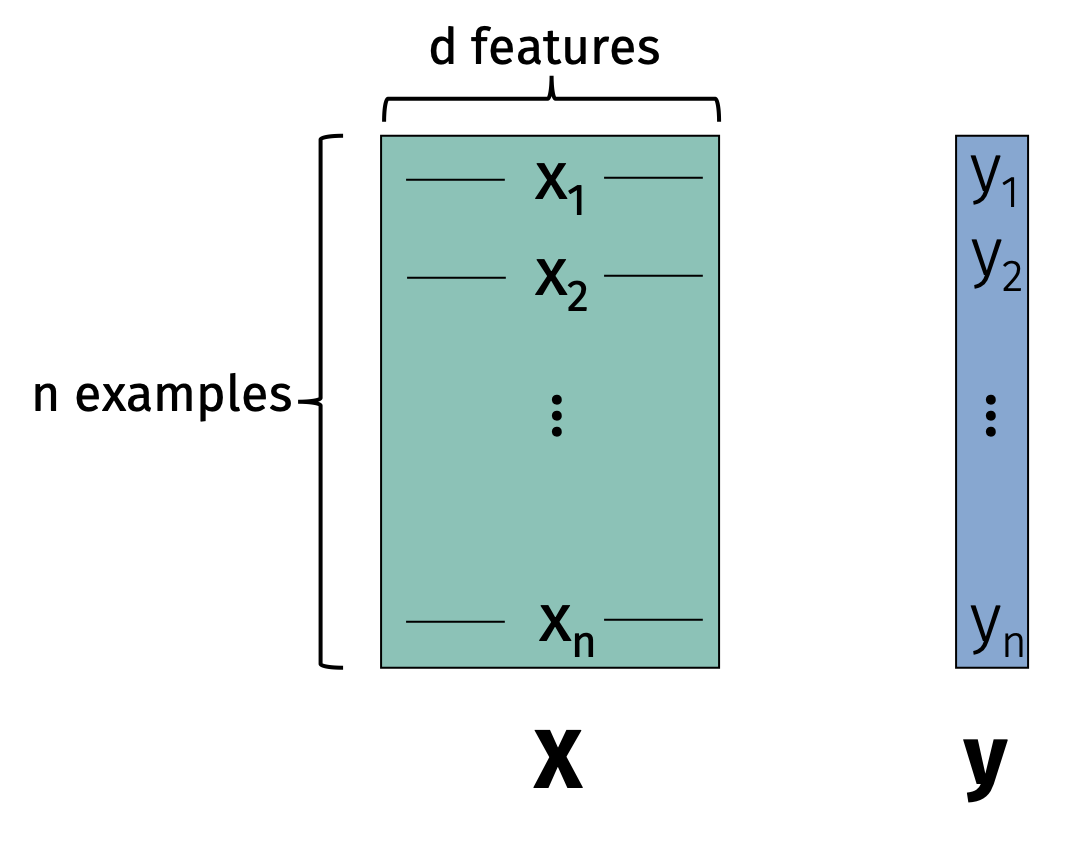
\includegraphics[width=.6\textwidth]{dataset.png}
	\end{center}
\end{frame}

\begin{frame}
	\frametitle{motivating example}
	\textbf{Motivating example:} Predict diabetes progression in patients after 1 year based on health metrics. (Measured via numerical score.) \vspace{1em}
	
	\textbf{Features:} Age, sex, body mass index, average blood pressure, six blood serum measurements (e.g. cholesterol, lipid levels, iron, etc.)
	
	\begin{center}
		Demo in \texttt{demo1\_diabetes.ipynb}. 
	\end{center}
\end{frame}

\begin{frame}
	\frametitle{the data matrix}
	\textbf{Predictor variables:}
	\begin{center}
		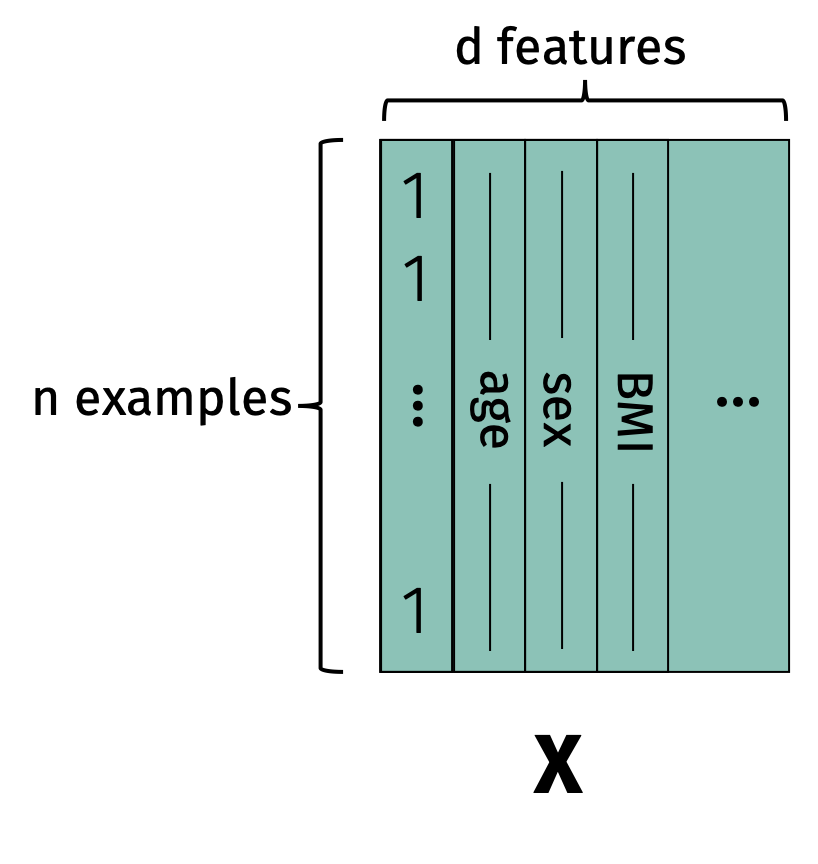
\includegraphics[width=.45\textwidth]{data_matrix_features.png}
	\end{center}
\end{frame}

\begin{frame}
	\frametitle{multiple linear regression}
	\begin{center}
		\textbf{Linear \emph{Least-Squares} Regression.}
	\end{center}
	\begin{itemize}
		\item Model: 
		\begin{align*}
		f_{\bs{\beta}}(\bv{x}) = \langle\bv{x},\bs{\beta}\rangle
		\end{align*}
		\item Model Parameters: 
		\begin{align*}
		\bs{\beta} = \left[\beta_1, \beta_2, \ldots, \beta_d \right]
		\end{align*}
		\item Loss Function:
		\begin{align*}
		L(\bs{\beta}) = \|\bv{y} -\bv{X}\bs{\beta}\|_2^2
		\end{align*}
	\end{itemize}
\end{frame}

\begin{frame}
	\frametitle{loss minimization}
	\textbf{Machine learning goal:} minimize the loss function $L(\bs{\beta}): \R^{d} \rightarrow \R$.
	
	\vspace{1em}
	Find optimum by determining for which $\bs{\beta} = [\beta_1, \ldots, \beta_d]$ the gradient is $0$. I.e. when do we have:
		\begin{align*}
		\nabla L(\beta) = \begin{bmatrix}
		 \frac{\partial L}{\partial \beta_1} \\ \frac{\partial L}{\partial \beta_2} \\ \vdots \\ \frac{\partial L}{\partial \beta_d}
		\end{bmatrix} = 
		\begin{bmatrix}
		0 \\ 0 \\ \vdots \\ 0
		\end{bmatrix} 
		\end{align*}
\end{frame}


\begin{frame}[t]
	\frametitle{gradient warmup}
	\textbf{Function:}
	\begin{align*}
	f(\bv{z}) = \bv{a}^T\bv{z} \text{ for some fixed column vector } \bv{a} \in \R^d
	\end{align*}
	
	\textbf{Gradient:}	\vspace{3em}
	
	\textbf{Function:}
	\begin{align*}
	f(\bv{z}) = \|\bv{z}\|_2^2
	\end{align*}
	
	\textbf{Gradient:}
	
\end{frame}

\begin{frame}[t]
	\frametitle{gradient warmup}
	\textbf{Function:}
	\begin{align*}
	f(\bv{z}) = g(\bv{A}\bv{z})= \text{ for fixed } \bv{A} \in \R^{n\times d} \text{ and function } g
	\end{align*}
	
	\textbf{Gradient:}	\vspace{3em}
	
	
\end{frame}

\begin{frame}[t]
	\frametitle{gradient}
	\textbf{Loss function:}
	\begin{align*}
	L(\bs{\beta}) = \|\bv{y} - \bv{X}\bs{\beta}\|_2^2
	\end{align*}
	
\end{frame}




\begin{frame}[t]
	\frametitle{gradient derivation}
	\begin{center}
	\textbf{Loss function:} $\|\bv{y} - \bv{X}\bs{\beta}\|_2^2$. 
	\end{center}
	
\end{frame}

\begin{frame}[t]
		\frametitle{loss minimization}
	\textbf{Goal:} minimize the loss function $L(\bs{\beta}) = \|\bv{y} - \bv{X}\bs{\beta}\|_2^2$.
	
	\begin{align*}
	\nabla L(\bs{\beta}) = 2\bv{X}^T\bv{X}\bs{\beta} - 2\bv{X}^T\bv{y} = \bv{0}
	\end{align*}
	
	\textbf{Solve for optimal $\bs{\beta}^*$:}
	\begin{align*}
	\bv{X}^T\bv{X}\bs{\beta}^* &= \bv{X}^T\bv{y} \\
	\alert{\bs{\beta}^*} &\alert{= \left(\bv{X}^T\bv{X}\right)^{-1}\bv{X}^T\bv{y}}
	\end{align*}
\end{frame}

\begin{frame}
	\frametitle{test your intuition}
	What is the sign of $\beta_1$ when we run a \emph{simple} linear regression using the following predictors for \emph{diabetes progression} in isolation:
	\begin{itemize}
		\item Body mass index (BMI): \textbf{Positive}
		\item Sex (values of 1 indicates male, value of 2 indicates female): \textbf{Positive}
	\end{itemize}
\end{frame}

\begin{frame}
	\frametitle{interacting variables}
	What is the sign of the corresponding $\beta$'s when we run a \emph{multiple} linear regression using the following predictors together:
\begin{itemize}
	\item Body mass index (BMI): \textbf{Positive}
	\item Sex (values of 1 indicates male, value of 2 indicates female): \textbf{Negative}
\end{itemize}
\begin{center}
	\alert{\textbf{Can you explain this? Try to think of your own example of a regression problem where this phenomenon might show up.}}
\end{center}
\end{frame}

\begin{frame}
	\frametitle{dealing with categorical variables}
	The \emph{sex} variable in the diabetes problem was \emph{binary}.
	
	Suppose we go back to the MPG prediction problem. What if we had a \emph{categorical} predictor variable for car make with more than 2 options: e.g. Ford, BMW, Honda. \textbf{How would you encode as a numerical column?}
	\begin{align*}
	\begin{bmatrix}
	\texttt{ford} \\\texttt{ford} \\ \texttt{honda} \\ \texttt{bmw} \\ \texttt{honda} \\ \texttt{ford}
	\end{bmatrix} \rightarrow 
	\begin{bmatrix}
	\hspace{2em} \\\hspace{2em} \\ \hspace{2em} \\ \hspace{2em} \\ \hspace{2em} \\ \hspace{2em}
	\end{bmatrix}
	\end{align*}
\end{frame}

\begin{frame}
	\frametitle{one hot encoding}
	\textbf{Better approach:} \emph{One Hot Encoding.}
	\begin{align*}
	\begin{bmatrix}
	\texttt{ford} \\\texttt{ford} \\ \texttt{honda} \\ \texttt{bmw} \\ \texttt{honda} \\ \texttt{ford}
	\end{bmatrix} \rightarrow 
	\begin{bmatrix}
	1 & 0 & 0 \\1 & 0 & 0 \\ 0 & 1 & 0 \\ 0 & 0 & 1\\ 0 & 1 & 0 \\ 1 & 0 & 0
	\end{bmatrix}
	\end{align*}
	\begin{itemize}
	\item Create a separate feature for every category, which is 1 when the variable is in that category, zero otherwise.
	\item Not too hard to do by hand, but you can also use library functions like \texttt{\small sklearn.preprocessing.OneHotEncoder}.
	\end{itemize}
	\begin{center}
		\large \alert{\textbf{Avoids adding inadvertent linear relationships.}}
	\end{center}
\end{frame}

\begin{frame}
	\frametitle{transformed linear models}
	Suppose we have singular variate data examples $(x, y)$. How could we fit the \emph{non-linear} model:
	\begin{align*}
	y \approx \beta_0 + \beta_1 x +  \beta_2 x^2 +  \beta_3 x^3.
	\end{align*}
	\begin{center}
		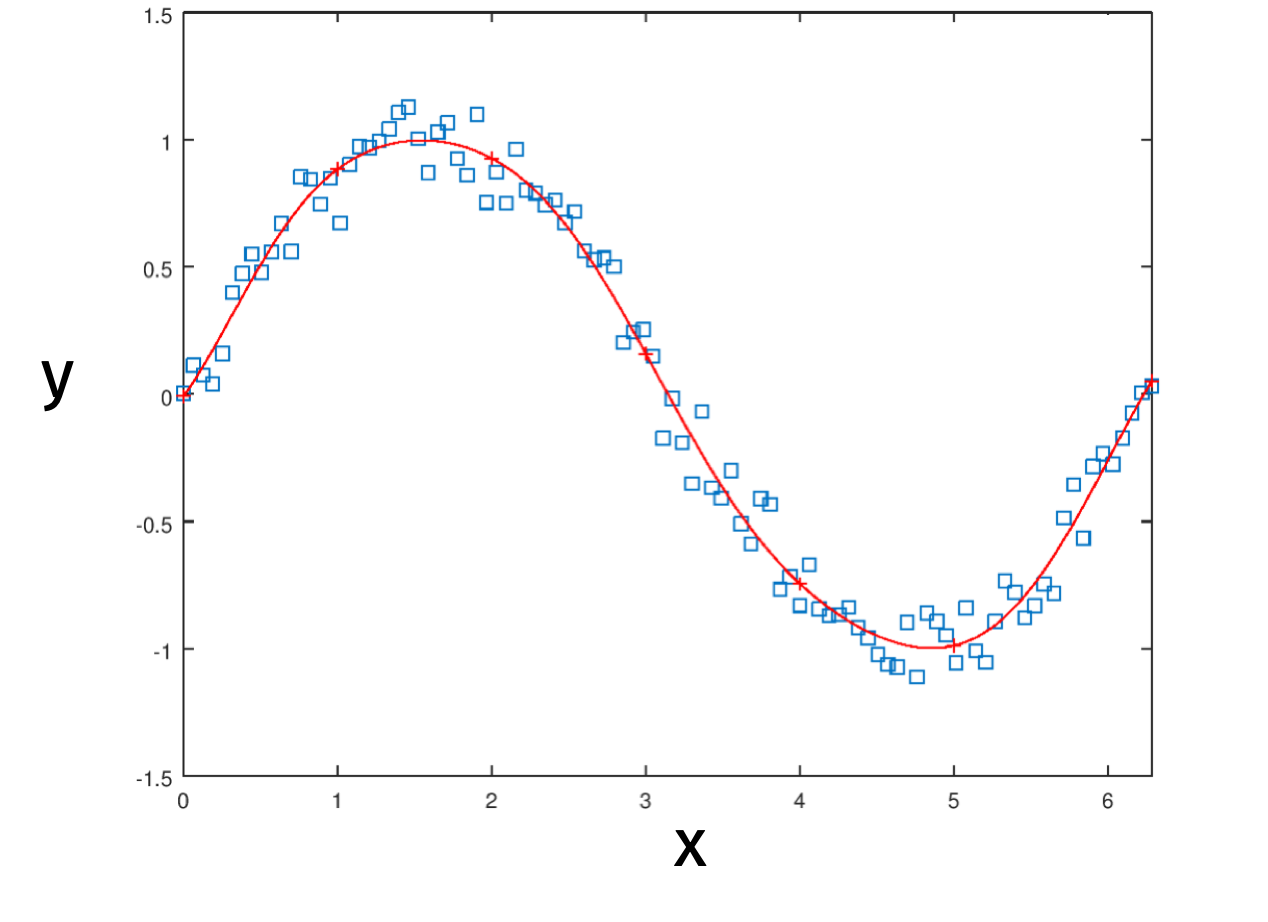
\includegraphics[width=.6\textwidth]{poly_fit.png}
	\end{center}
\end{frame}

\begin{frame}
	\frametitle{transformed linear models}
	Transform into a multiple linear regression problem:
	\begin{align*}
	\textbf{X} = \begin{bmatrix}
	1 & x_1  &  x_1^2 & x_1^3\\
	1 & x_2  &  x_2^1 &  x_2^3 \\
	1 & x_3  &  x_3^2 &  x_3^3\\
	\vdots & \vdots  &  &\vdots\\
	1 & x_n  &  x_n^2 & x_n^3\\ 
	\end{bmatrix}
	\end{align*}
	Each column $j$ is generated by a different basis function $\phi_j(x)$. Could have:
	\begin{itemize}
		\item $\phi_j(x) = x^q$
		\item $\phi_j(x) = sin(x)$
		\item $\phi_j(x) = cos(10x)$
		\item $\phi_j(x) = 1/x$
	\end{itemize}
\end{frame}

\begin{frame}
	\frametitle{transformed linear models}
	\begin{center}
		\textbf{Transformations can also be for multivariate data.}
	\end{center}
	\textbf{Example:} Multinomial model.
	\begin{itemize}
		\item Given a dataset with \emph{target $y$} and \emph{predictors $x, z$}.
		\item For inputs $(x_1,z_1), \ldots, (x_n,z_n)$ construct the data matrix:
		\begin{align*}
		\begin{bmatrix}
		1 & x_1  &  x_1^2 & z_1 & z_1^2 & x_1z_1\\
		1 & x_2  &  x_2^2 & z_2 & z_2^2 & x_2z_2\\
		\vdots & \vdots  &  &\vdots\\
		1 & x_n  &  x_n^2 & z_n & z_n^2 & x_nz_n\\
		\end{bmatrix}
		\end{align*}
		\item Captures non-linear interaction between $x$ and $y$.
	\end{itemize}
\end{frame}

\begin{frame}
	\frametitle{model selection}
	\textbf{Remainder of lecture:}
	Learn about \emph{model selection}, \emph{test/train paradigm}, and \emph{cross-validation} through a simple example.
	
s\end{frame}

\begin{frame}
	\frametitle{fitting a polynomial}
	\textbf{Simple experiment:} 
	\begin{itemize}
	\item Randomly select data points $x_1, \ldots, x_n \in [-1,1]$.
	\item Choose a degree 3 polynomial $p(x)$. 
	\item Create some fake data: $y_i = p(x_i) + \eta$ where $\eta$ is a random number (e.g random Gaussian).
	\end{itemize}
	\begin{center}
		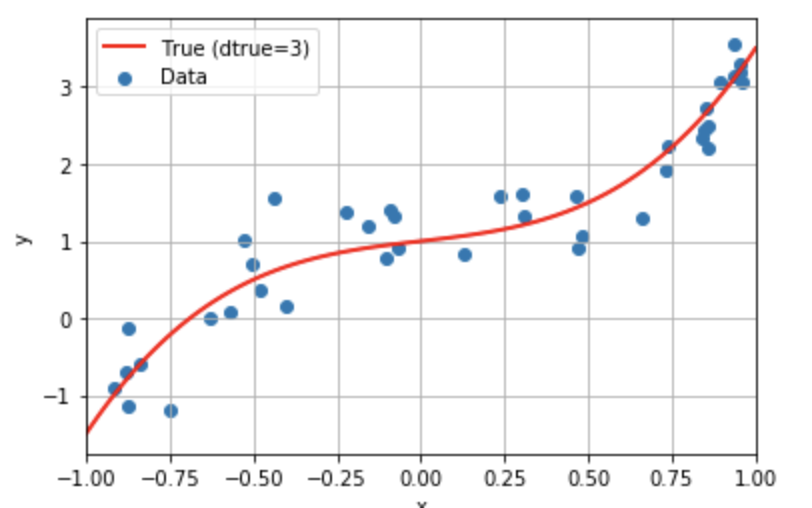
\includegraphics[width=.5\textwidth]{data.png}
	\end{center}
\end{frame}

\begin{frame}
	\frametitle{fitting a polynomial}
	\textbf{Simple experiment:} 
	\begin{itemize}
		\item Use multiple linear regression to fit a degree $3$ polynomial.
	\end{itemize}
	\begin{center}
		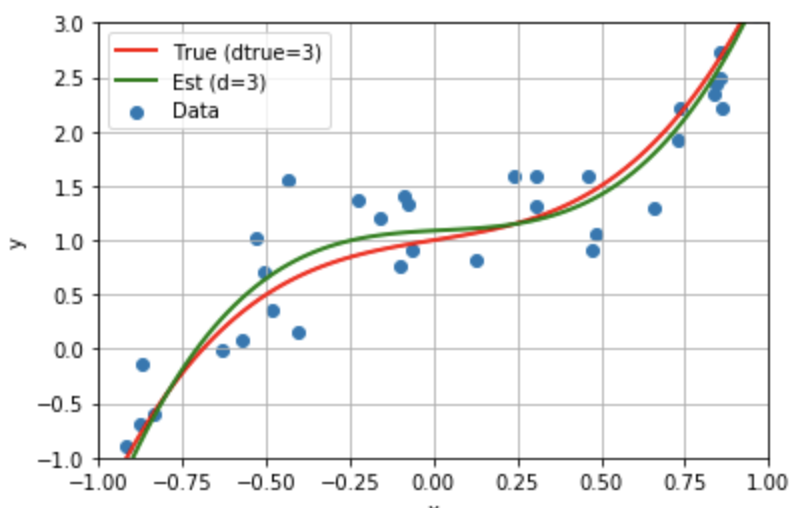
\includegraphics[width=.5\textwidth]{fit3.png}
	\end{center}
\end{frame}

\begin{frame}
	\frametitle{fitting a polynomial}
	\textbf{What if we fit a higher degree polynomial?} 
	\begin{itemize}
		\item Fit degree $5$ polynomial under squared loss.
		\item Fit degree $10$ polynomial under squared loss.
	\end{itemize}
	\begin{center}
		\includegraphics[width=.5\textwidth]{fit5.png}\includegraphics[width=.5\textwidth]{fit10.png}
	\end{center}
\end{frame}

\begin{frame}
	\frametitle{fitting a polynomial}
	\textbf{Even higher?} 
	\begin{itemize}
		\item Fit degree $40$ polynomial under squared loss.
	\end{itemize}
	\begin{center}
		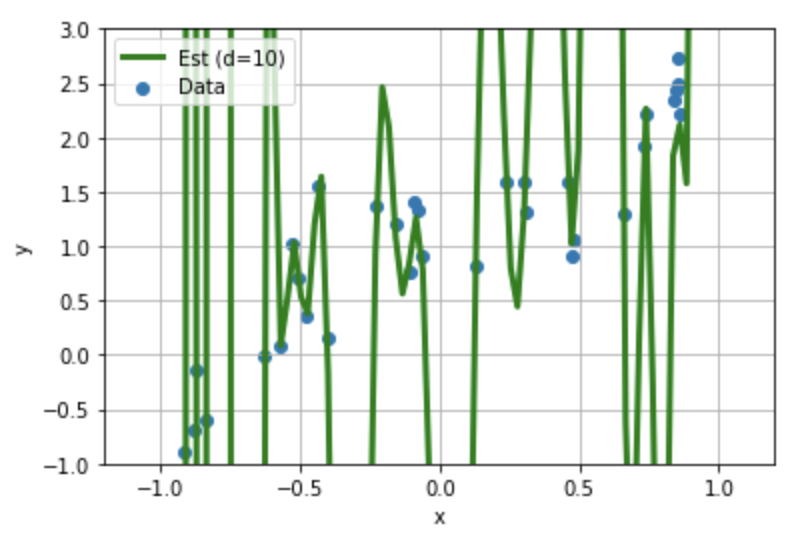
\includegraphics[width=.5\textwidth]{fit40.png}
	\end{center}
\end{frame}

\begin{frame}
	\frametitle{model selection}
	The more \textbf{complex} our model class (i.e. the higher degree we allow) the better our loss:
	\begin{center}
		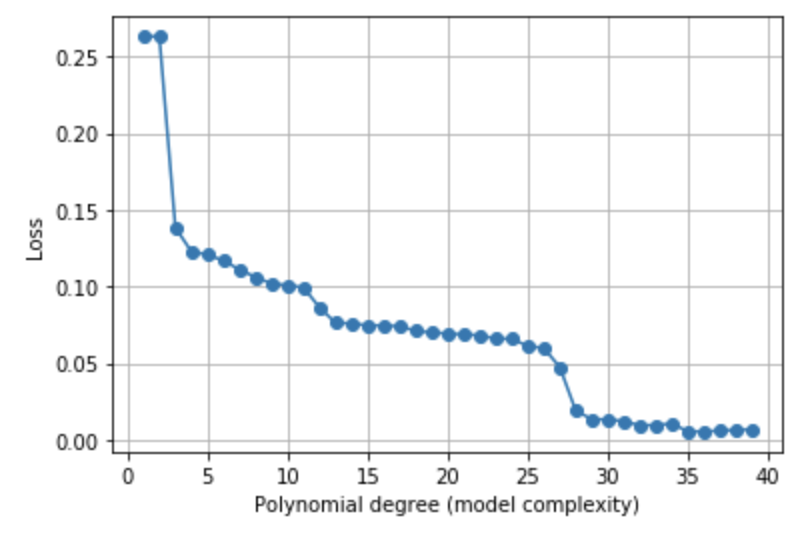
\includegraphics[width=.5\textwidth]{loss.png}
		
		\alert{\textbf{Is our model getting better and better?}}
		
		\textbf{Given the raw data, how do we know which model to choose? Degree 3? Degree 5? Degree 40?}
	\end{center}
\end{frame}

\begin{frame}
	\frametitle{model selection}
	\textbf{Problem:} Loss alone is not informative for choosing model.
	
	For more complex models, we get smaller loss on the training data, but don't expect to perform well on ``new'' data:
	\begin{center}
		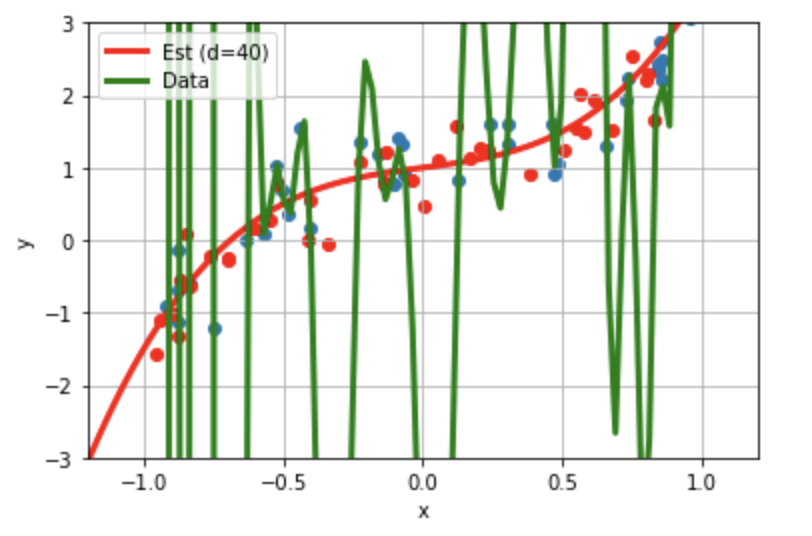
\includegraphics[width=.5\textwidth]{newdata.png}
	\end{center}

In other words, the model does not \alert{\textbf{generalize.}}
	
%	\textbf{Solution:} Directly check how our model would perform on ``new data''. I.e. how well does the model \emph{generalize}.
\end{frame}

\begin{frame}
	\frametitle{model selection}
	\textbf{Solution:} Directly test model on ``new data''.
	
	\begin{center}
		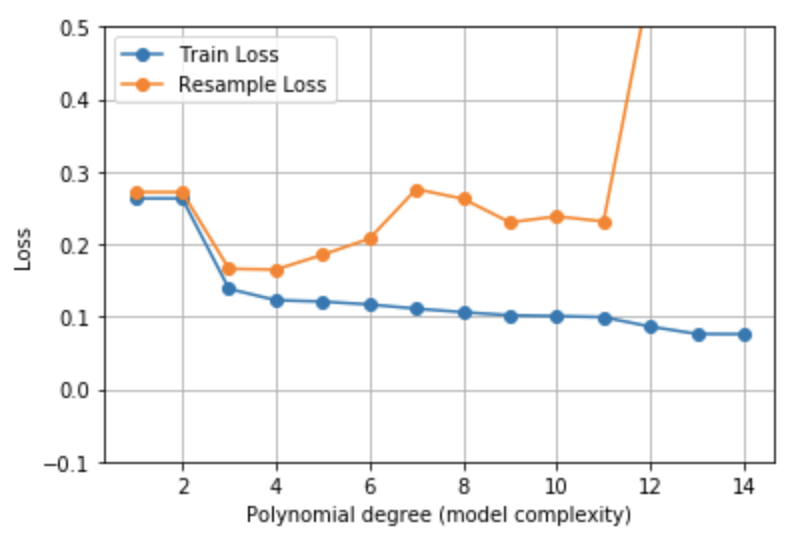
\includegraphics[width=.6\textwidth]{generalization.png}
	\end{center}
\begin{itemize}
	\item Loss continues to decrease as model complexity grows.
	\item Performance on new data ``turns around'' once our model gets too complex. Minimized around degree $4$.
\end{itemize}
\end{frame}

\begin{frame}
	\frametitle{train-test paradigm}
	 In most situations, we cannot simply collect or generate ``new data''. Here's an alternative:
	 
	 \textbf{Test/train split:}
	 \small
	\begin{itemize}
		\item Given data set $(\bv{X}, \bv{y})$, split into two sets $(\bv{X}_{tr}, \bv{y}_{tr})$ and $(\bv{X}_{ts}, \bv{y}_{ts})$.
		\item Train $q$ models $f_1, \ldots, f_q$ by finding parameters which minimize the loss on $(\bv{X}_{tr}, \bv{y}_{tr})$.
		\item Evaluate loss of each trained model on $(\bv{X}_{ts}, \bv{y}_{ts})$.
	\end{itemize}
\end{frame}

\begin{frame}
	\frametitle{train-test paradigm}
	\small
	\textbf{Justification:}
	\begin{itemize}
		\item Assume each data example is randomly drawn from some distribution $(\bv{x},y)\sim \mathcal{D}$: we don't care about any particulars of this distribution.
		\item \textbf{Goal:} Find model $f \in \{f_1, \ldots, f_q\}$ and parameter vector $\bs{\theta}$ to minimize the \alert{\textbf{Risk}}:
		\begin{align*}
			R(f,\bs{\theta}) = \E_{(\bv{x},y)\sim\mathcal{D}} \left[L\left(f(\bv{x},\bs{\theta}) - y\right) \right]
		\end{align*}
		where $L$ is some loss function (e.g. $L(z) = |z|$ or $L(z) = z^2$).
	\end{itemize}
\end{frame}

\begin{frame}
	\frametitle{train-test paradigm}
	\small
	\textbf{Justification:}
	\begin{itemize}
		\item Suppose the testing dataset $(\bv{X}_{ts}, \bv{y}_{ts})$ has $m$ examples.
		\item Given any model $f$ and parameters $\bs{\theta}$, let 
		\begin{align*}
			L_{ts}(f,\bs{\theta}) = \frac{1}{m}\sum_{\bv{x},y \in (\bv{X}_{ts}, \bv{y}_{ts})} L\left(f(\bv{x},\bs{\theta}) - y\right)
		\end{align*}
		\item \textbf{Claim:}\footnote{Only true if $f$ and $\bs{\theta}$ are chose \textit{without looking at your test data.}}
		\begin{align*}
		\E\left[L_{ts}(f,\bs{\theta})\right] = R(f,\bs{\theta}).
		\end{align*}
		\item So our testing error is an \emph{unbiased estimate} for the true \emph{risk} which measures how well a function performs on average for any ``new'' data point.
	\end{itemize}
\vspace{1em}
\end{frame}

\begin{frame}
	\frametitle{how to split data}	
	How should  be divide up our data into training and test data?
	\begin{itemize}
		\item 50\% train, 50\% test?
		\item 80\% train, 20\% test?
		\item 20\% train, 80\% test?
	\end{itemize}
	There is a trade-off here. A larger test set allows for a more accurate estimate of the risk $R$, which helps us choose as model. However, it means we have less data to train with, so for each individual model we might get a worst set of parameters.
\end{frame}

\begin{frame}
	\frametitle{k-fold cross validation}
	\begin{center}
		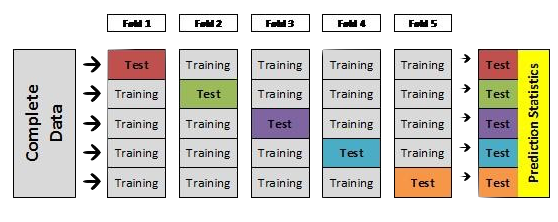
\includegraphics[width=.7\textwidth]{crossval.png}
	\end{center}
	\begin{itemize}
		\item Randomly divide data in $K$ parts. 
		\begin{itemize}
			\item Typical choice: $K = 5$ or $K = 10$.
		\end{itemize}
		\item Use $K-1$ parts for training, $1$ for test.
		\item For each model, compute test loss $L_{ts}$ for each ``fold''.
		\item Choose model with best average loss. 
		\item Retrain best model on entire dataset.
	\end{itemize}
\end{frame}

\begin{frame}
	\frametitle{k-fold cross validation}
	\textbf{Leave-one-out cross validation}: take $K = n$, where $n$ is our total number of samples. 
	
	\begin{center}
		\alert{\textbf{Is there any disadvantage to choosing $K$ larger?}}
	\end{center}
	
\end{frame}

\end{document} 








